\documentclass{article}
\usepackage{array, tabularx}
\usepackage{pdfpages}

\newcolumntype{Y}{>{\centering\arraybackslash}X}

\newdimen\demilargeur
\demilargeur=\textwidth
\divide\demilargeur by 2
\newcommand\tab[1][1cm]{\hspace*{#1}}

\title{Protocoles de communication graphique 2D}
\date{}
\begin{document}
\maketitle
\part*{Introduction}
Protocoles de communication graphique 2D ou Code barre  bidimensionnel  ou Codes matriciels\\
Les protocoles de communication graphique [...]\\
Les codes barres [...]\\
Les codes 2D [ Qr code...]\\
\part*{Sujet}
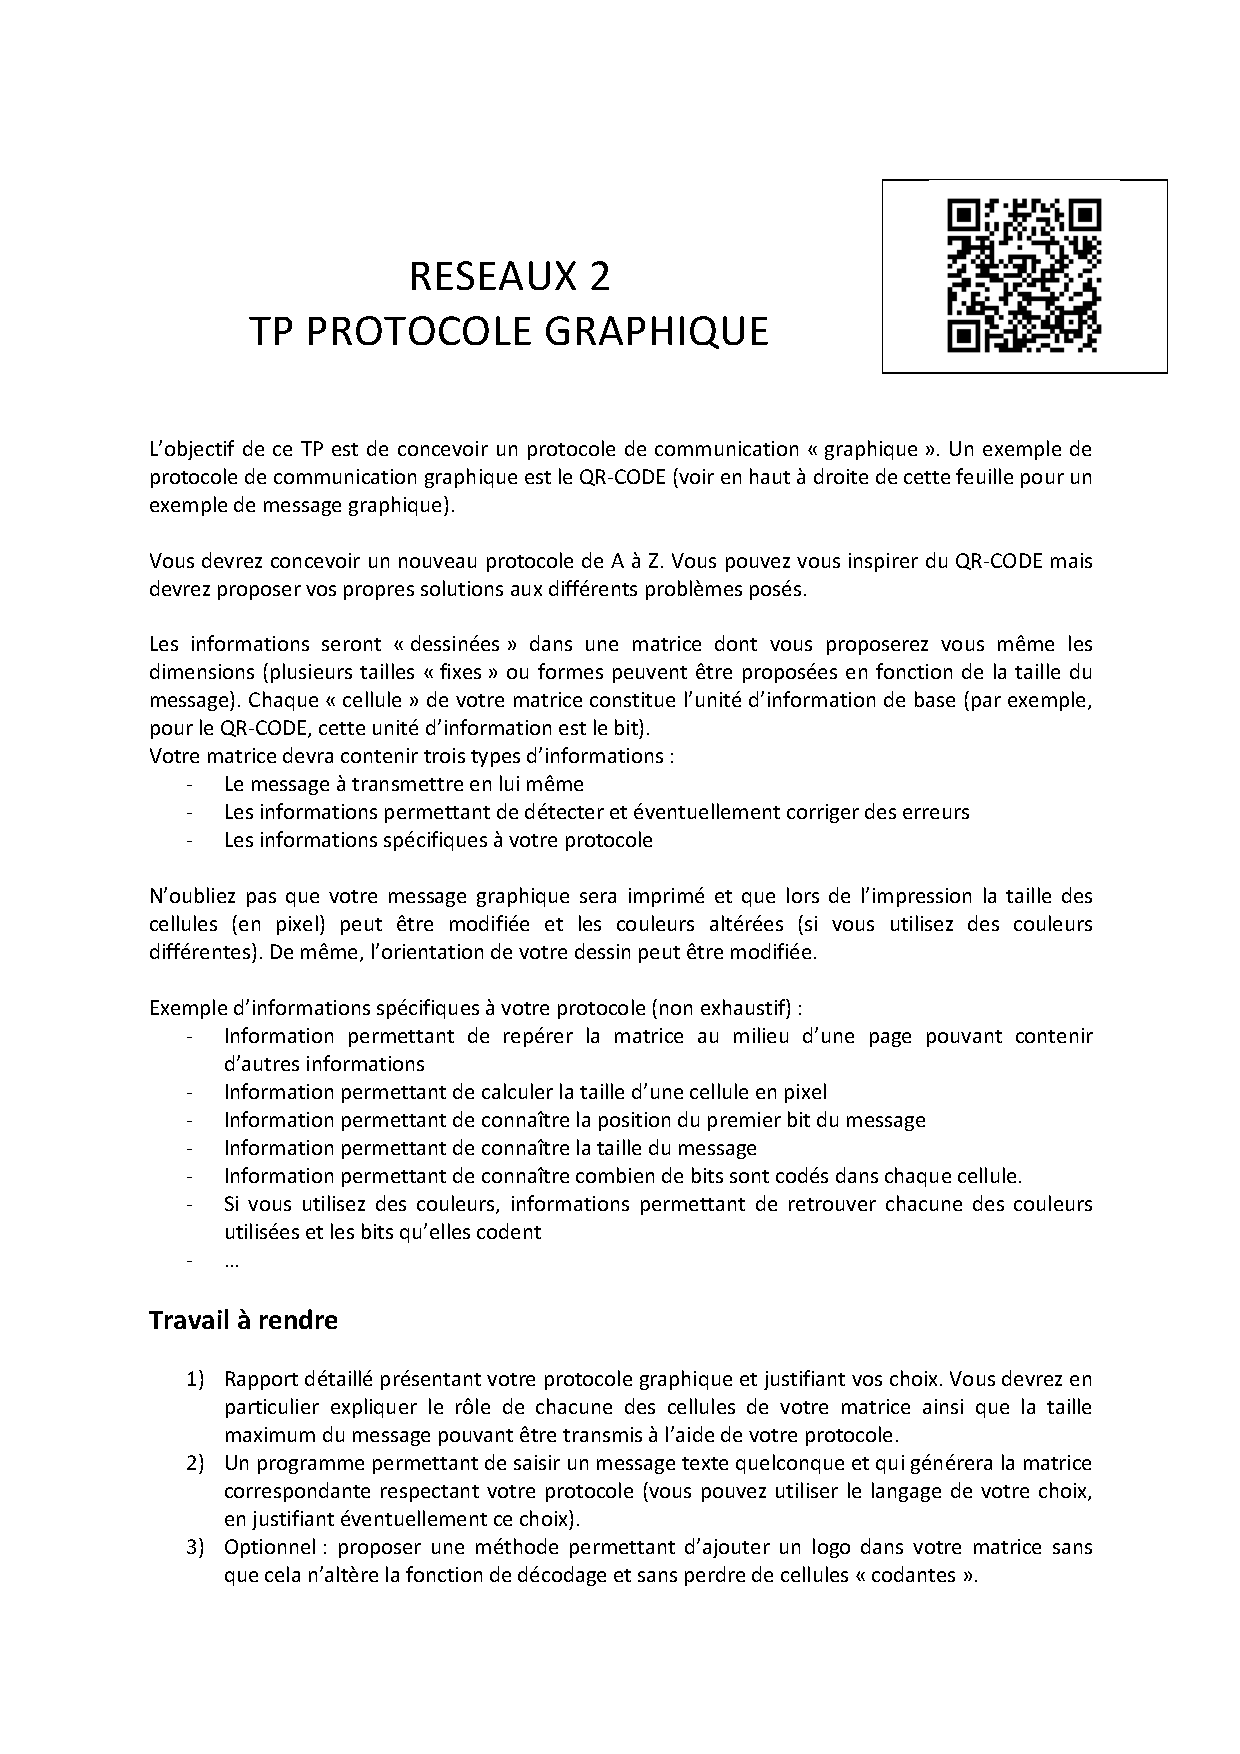
\includepdf[scale=0.80]{TPReseaux2.pdf}
\part{Fonctionnement}

$\bullet$ 1 - Analyse des données à encoder et paramétrage du niveau de code correcteur.
             Si pas de niveau de code correcteur spécifié $\rightarrow$ plus petite version de QR Code.\\
\\
$\bullet$ 2 - Convertion des données dans un flux de bytes.\\
    encodage des donnees (+ concatenation)\\
	ajout complementaire\\
		indicateur de mode (alpha numeric,...) 4bits\\
		nombre de caractere [...]\\
	Edition du code de correction d'erreur $\rightarrow$ choisir niveau de correction\\
	creation structure messages finale (block d'info/bits)\\
\\
$\bullet$ 3 - Implémentation de la correction des erreurs.
         séparation en blocs des bits de données et géneration du codes correcteurs.\\
	$\tab$(Capacité à corriger les erreurs :\\
    $\tab$Niveau L : environ 7 \% de redondance\\
    $\tab$Niveau M : environ 15 \%\\
    $\tab$Niveau Q : environ 25 \%\\
    $\tab$Niveau H : environ 30 \%\\
    $\tab$-Code correcteur, code de Redd Solomon (et Code de Hamming ))\\
\\
$\bullet$ 4 - Insérer les données avec le code correcteur dans la matrice.\\
    
    Utilisation de masque de patterns (Timing pattern, pattern de detection, pattern d'alignement)\\
    
	Placement des éléments:\\
		$\rightarrow$ motifs de positionnement\\
		les séparateur (pour distinguer les motifs de pos)\\
		$\rightarrow$ motifs de synchonisation/Timming patterns permettant de percevoir les contrastes entre les modules (clairs et foncés) et il permettent de determiner la version du Qr code (avec ça taille)\\
		$\rightarrow$ motifs de d'alignement (pareil mais plus petit que les motifs de positionnement), facilite la lecture en cas de deformation de la matrice.\\
	$\rightarrow$ zone tranquille autour du symbol/matrice.\\
	$\rightarrow$Placement des info/codewords\\
\\
$\bullet$ 5 - Génération de la matrice et évaluation du résultat retourné.\\
             optimisisation de la balance entre les modules noirs et les modules blancs et minimisation des occurrences de patterns indésirables\\
	$\tab$Creation du masque\\
	$\tab$Application du masque\\
	$\tab$Informations de format\\
	$\tab$Informations de version\\
\\
$\bullet$ 6 - Génération du QR Code au format image.\\
\\
(lecture\\
    $\tab$1 - Reconnaître les bits 1 ou 0.\\
             Le but est de différencier les modules noirs des modules blancs.\\
    $\tab$2 - Identifier le taux de code correcteur.\\
    $\tab$3 - Identifier la version du QR Code.\\
    $\tab$4 - Découvrir la région à décoder.\\
    $\tab$5 - Lire les données et le code correcteur.\\
    $\tab$6 - Détecter/Corriger les erreurs.\\
    $\tab$7 - Décoder les données.\\
    $\tab$8 - Afficher le résultat.\\
)\\
\\
Exemple : ZXing Open source en java\\

\part{Mise en place}
Le langage uilisé est java, avec swing. Le logiciel est développé sous Intel ij. (a mettre dans utilisation ?)
\subsection{Encodage et versionnage:}
...
\\
\subsection{Convertion:}
...
\\
\subsection{Code correcteur:}
...
\\
\subsection{Insertion (les differents motifs):}
$\tab$Contour faisant zone tranquille/tampon\\
...
\\
\subsection{ generation matrice ( masque,format,version) :}
...
\\
\subsection{Generation Code 2D:}
...
\\

\part{Utilisation}
\subsection{Compilation:}
\subsection{Execution:}

\end{document}